\documentclass[a4wide, 10pt]{article}
\usepackage{a4, fullpage}
\usepackage[pdftex]{graphicx}  
\usepackage[export]{adjustbox}
\usepackage{caption}
\usepackage{subcaption}
\setlength{\parskip}{0cm}
\setlength{\parindent}{1em}

% This is the preamble section where you can include extra packages etc.

\begin{document}

\title{Project Management Report}

\author{Cardspark - Group 26}

\date{\today}         % inserts today's date

\maketitle            % generates the title from the data above

\paragraph{Start of iteration}
Slack is how we communicate between each other and has apps like Trello, Github and CircleCI integrated with it.  Trello is our note leaving app where we post tasks of what we need to do for each iteration.  At this stage we mainly post ideas in Slack and what we need to do for the week in Trello.
\begin{figure}[h]
\centering
\begin{subfigure}{.5\textwidth}
  \centering
  	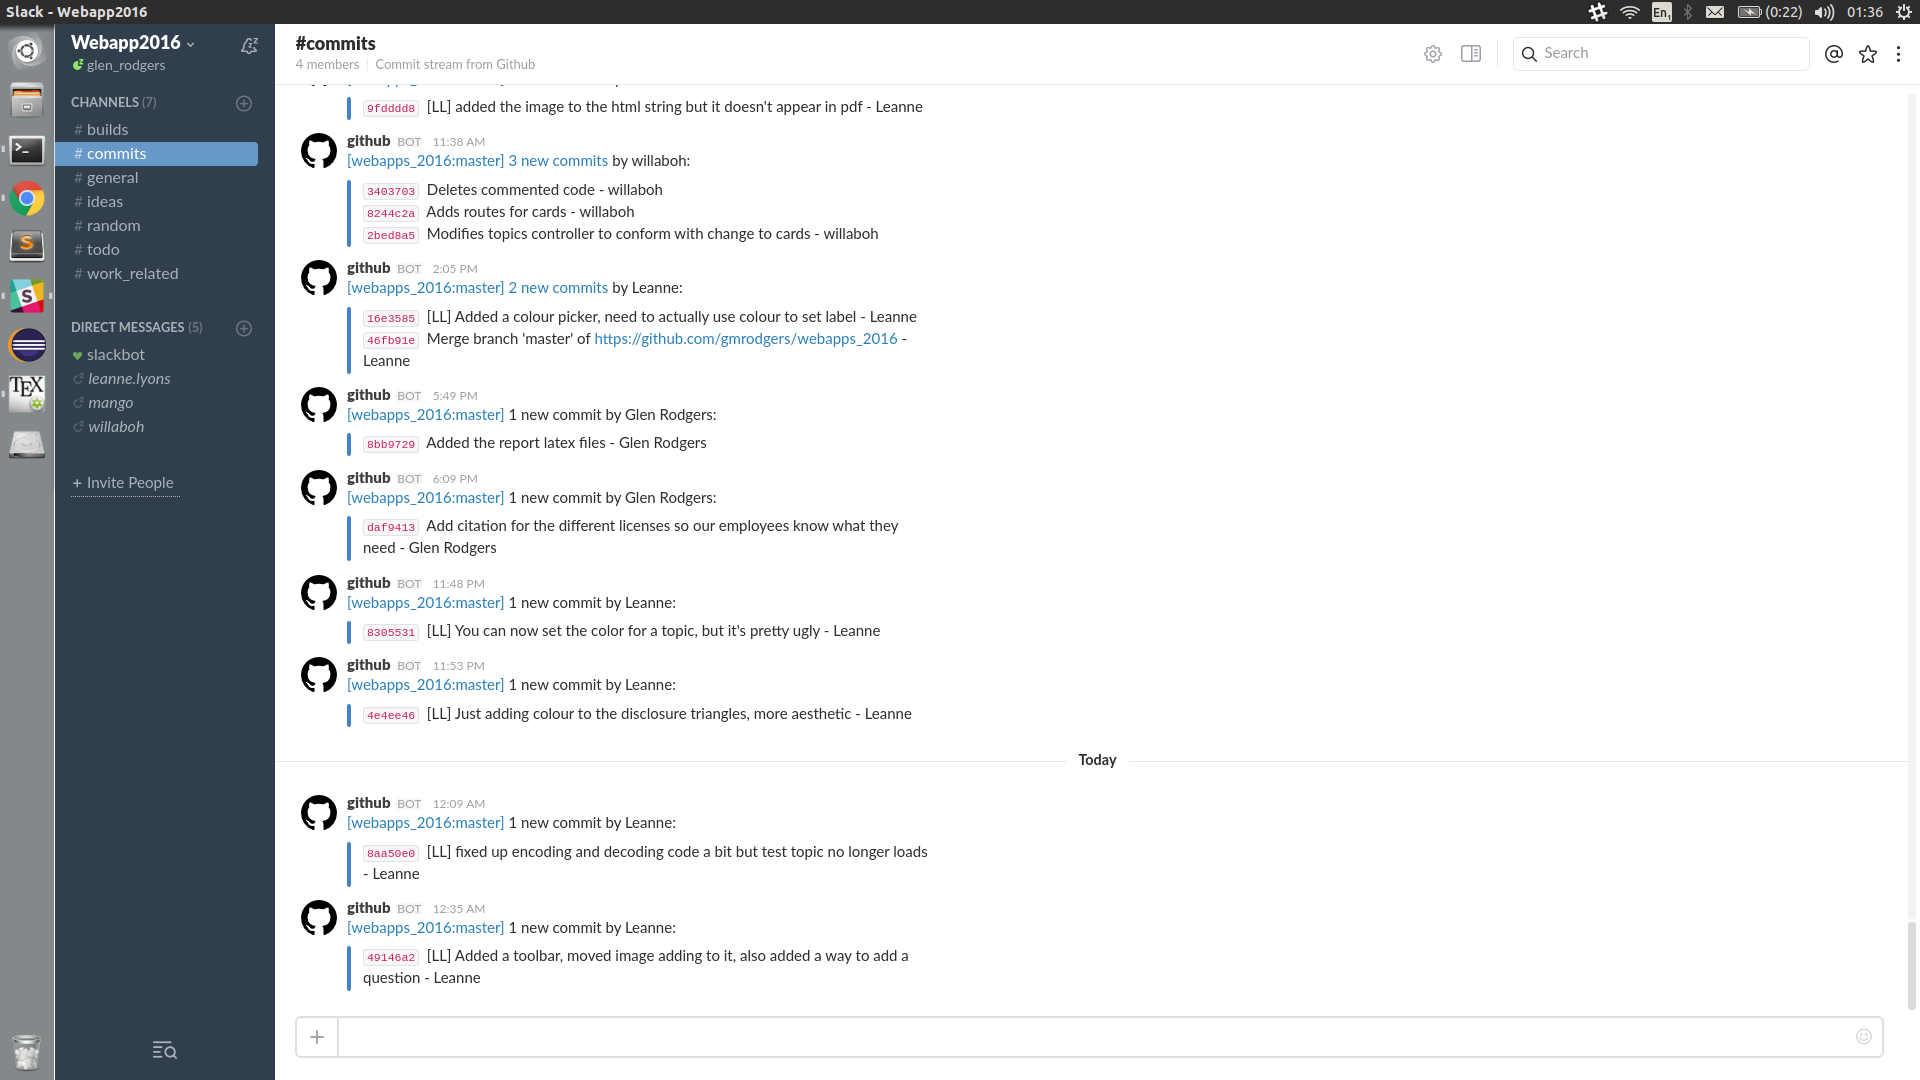
\includegraphics[scale=0.1]{slackstart.png} 
  \caption{Slack App}
  \label{fig:sub1}
\end{subfigure}%
\begin{subfigure}{.5\textwidth}
  \centering
  	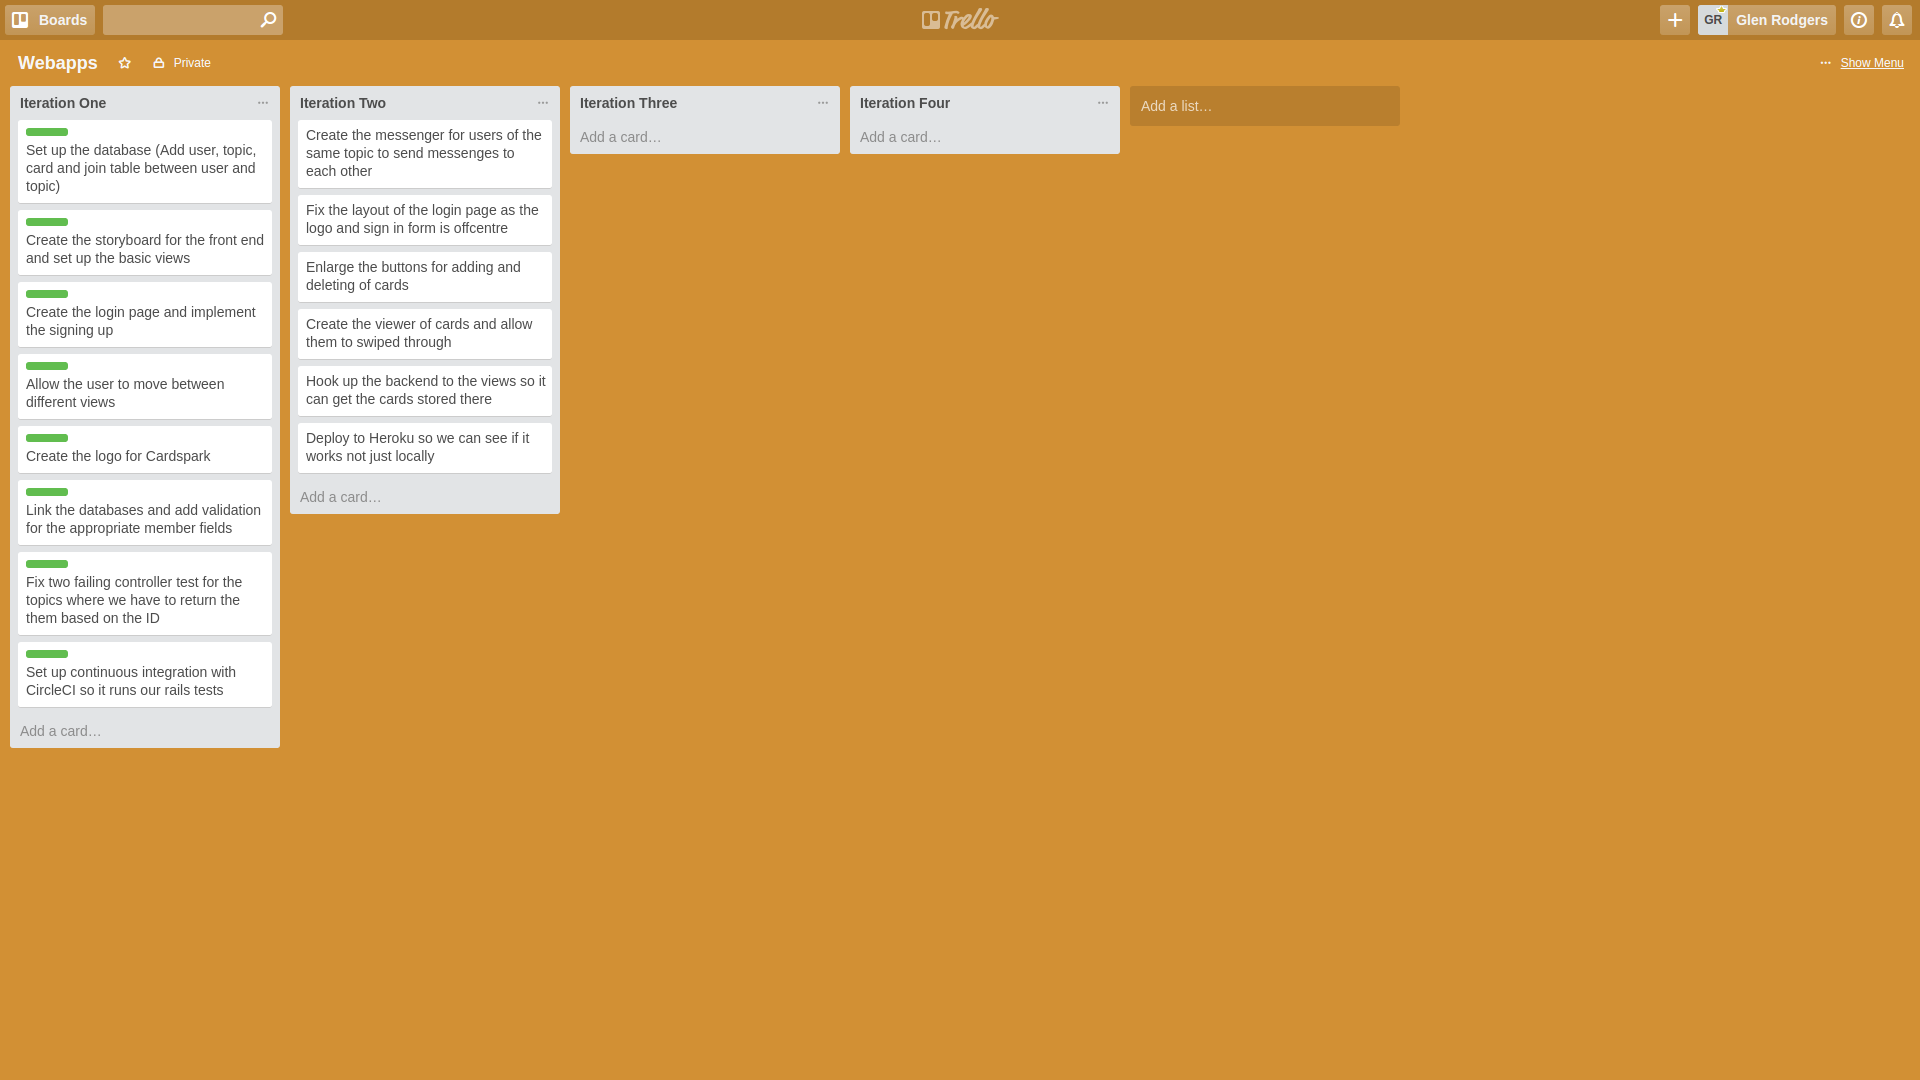
\includegraphics[scale=0.1]{iterationstart.png} 
  \caption{Trello App}
  \label{fig:sub2}
\end{subfigure}
\label{fig:test}
\end{figure}
\vspace*{-\baselineskip} 

\vspace{-0.3cm}
\paragraph{Middle of iteration} 
Slack is now used mainly for work queries and discussions instead of idea generation and user feedback.  Most of the cards should be marked as finished and we are now working on.
\begin{figure}[h]
\centering
\begin{subfigure}{.5\textwidth}
  \centering
  	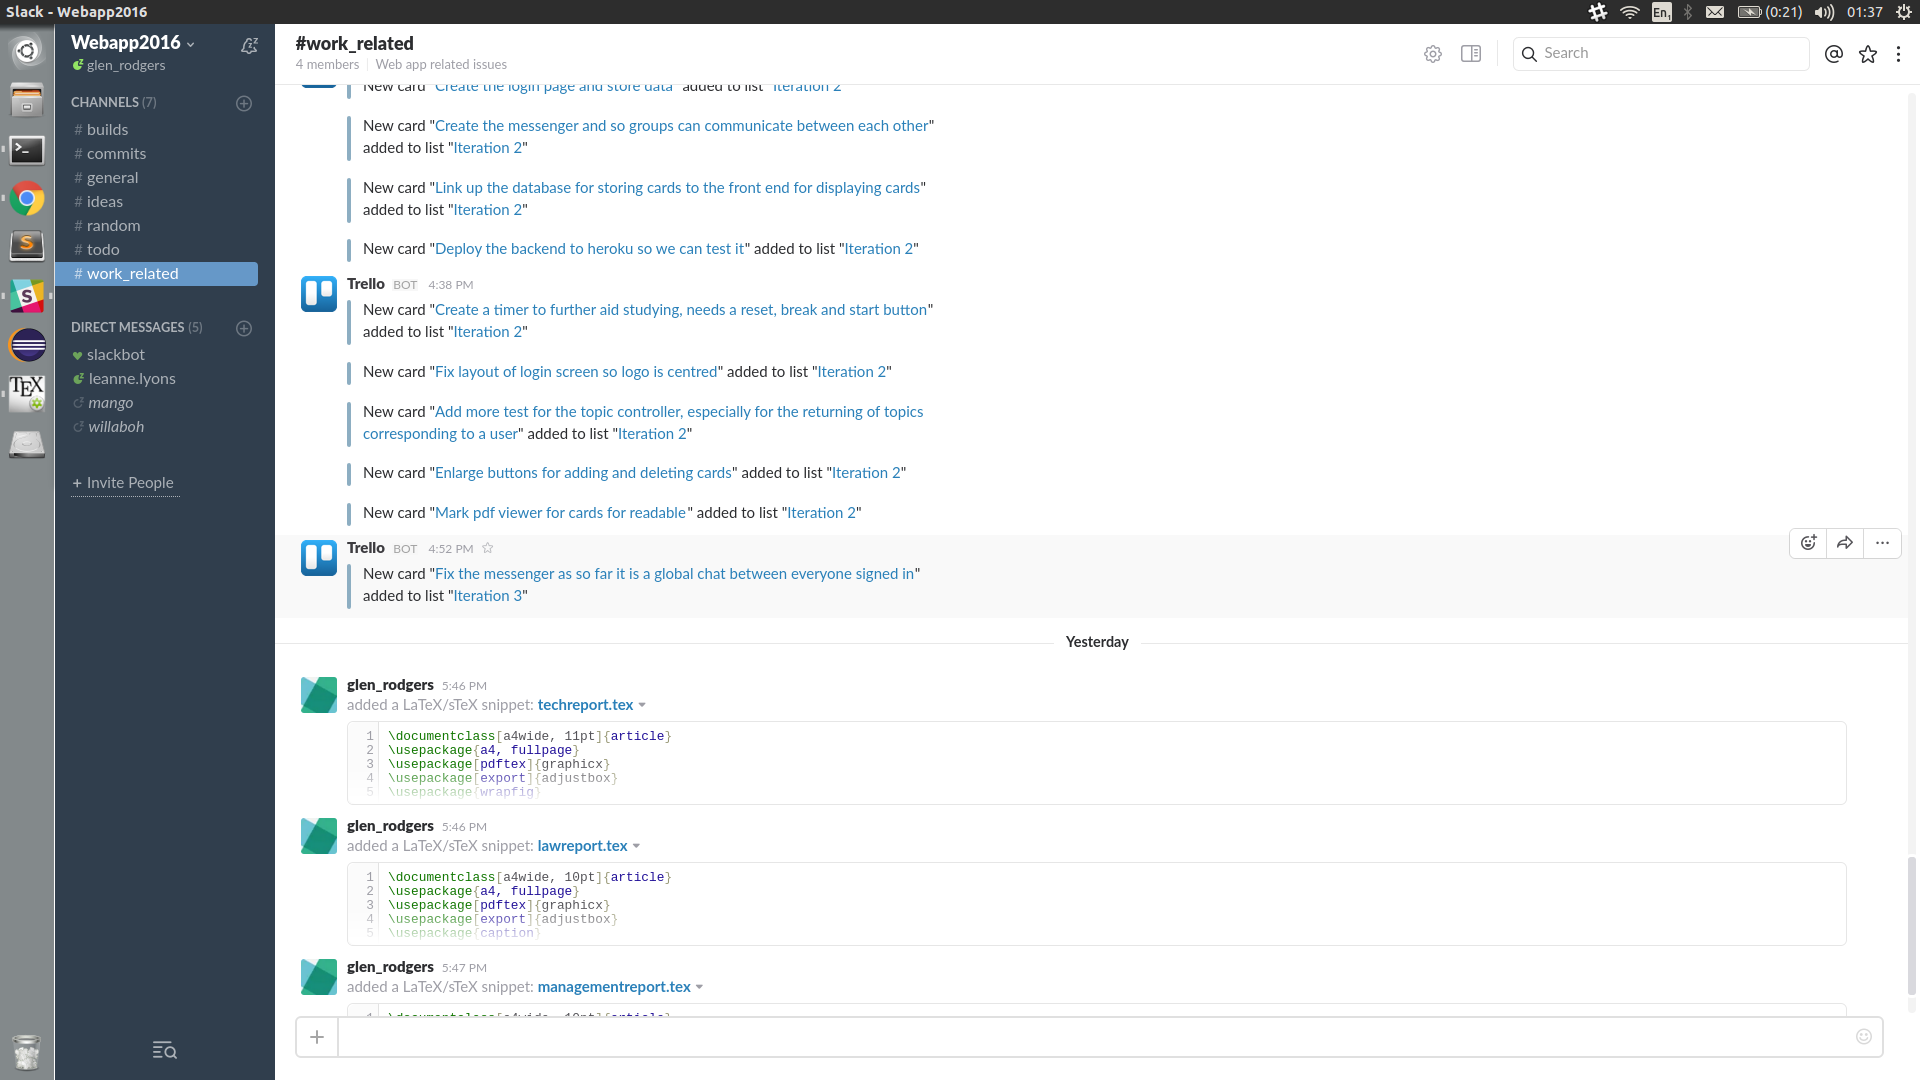
\includegraphics[scale=0.1]{slackmiddle.png} 
  \label{fig:sub1}
\end{subfigure}%
\begin{subfigure}{.5\textwidth}
  \centering
  	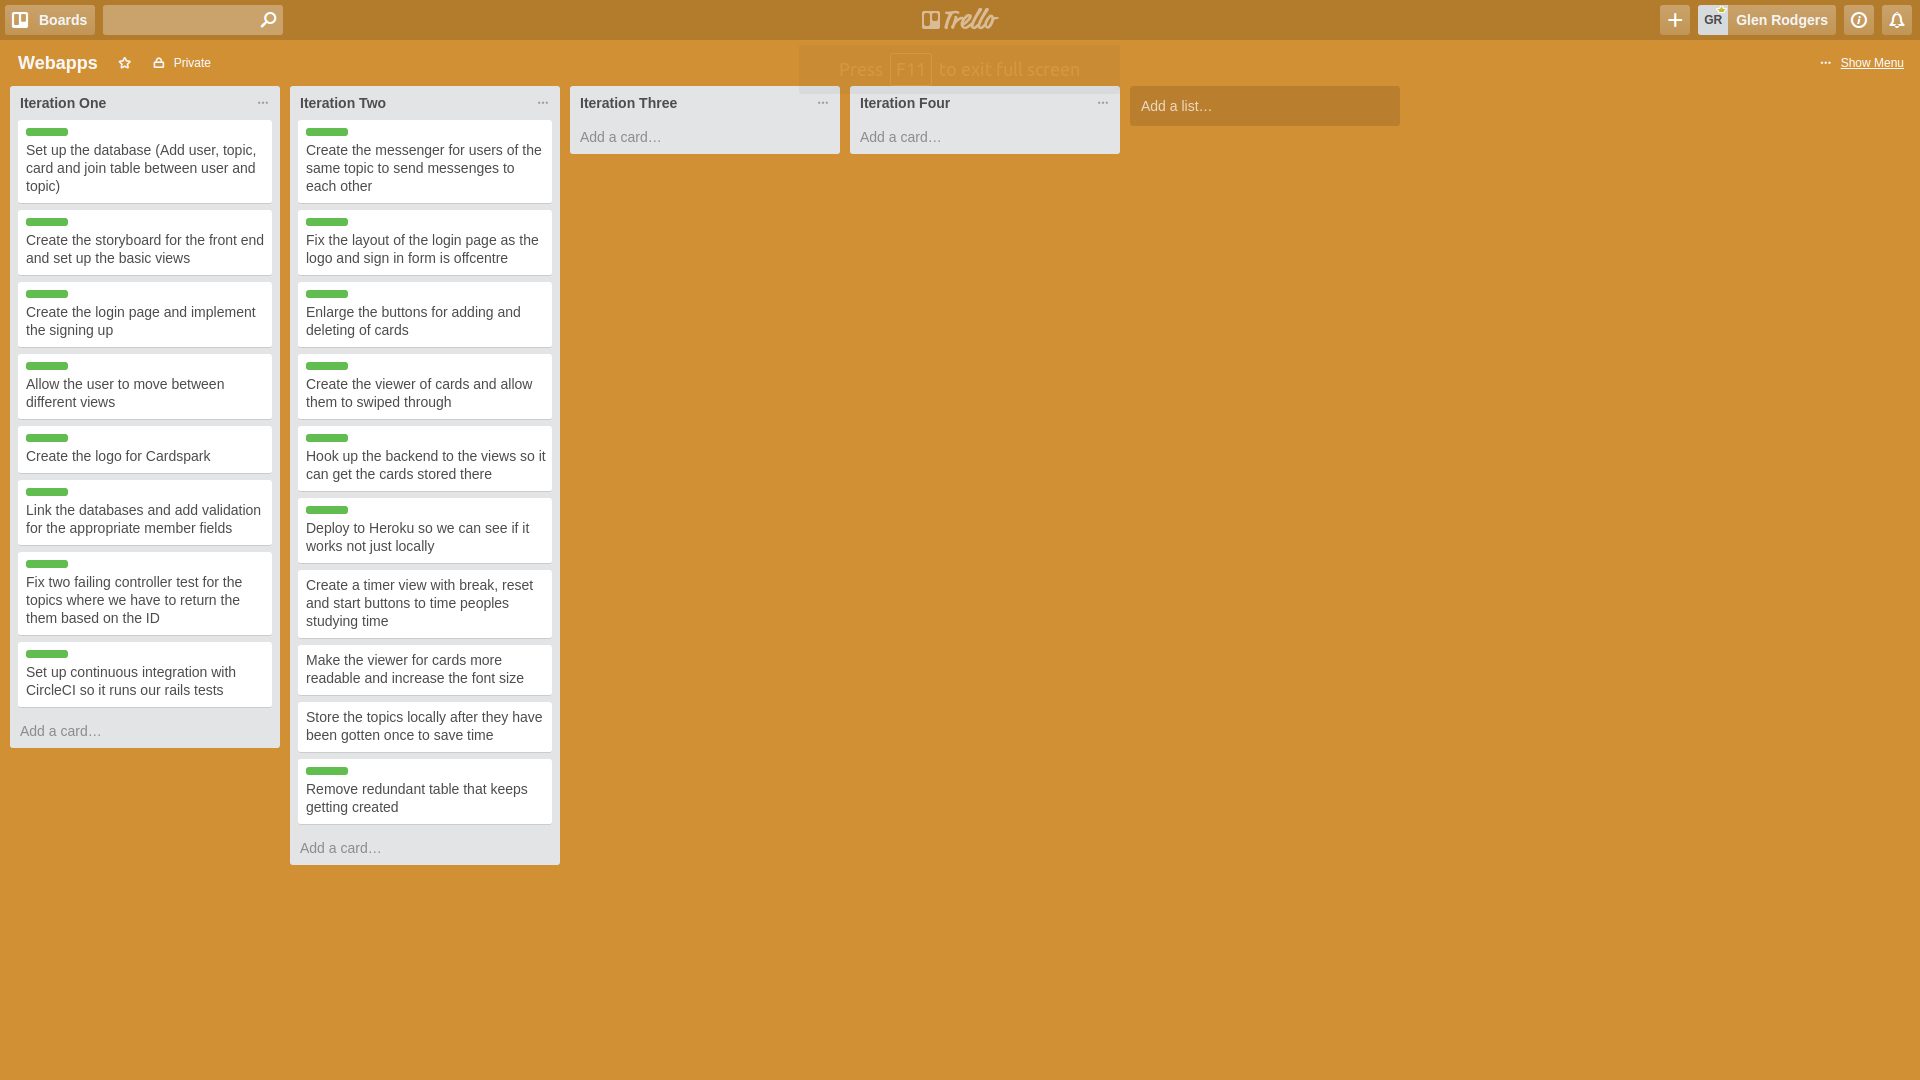
\includegraphics[scale=0.1]{iterationmiddle.png} 
  \label{fig:sub2}
\end{subfigure}
\label{fig:test}
\end{figure}
\vspace*{-\baselineskip} 

\vspace{-0.3cm}
\paragraph{End of iteration}
In Slack, the focus is now on the work-related channel completely as well as the builds and commits channels.  Cards are now marked as finished or moved to the next iteration.
\begin{figure}[h]
\centering
\begin{subfigure}{.5\textwidth}
  \centering
  	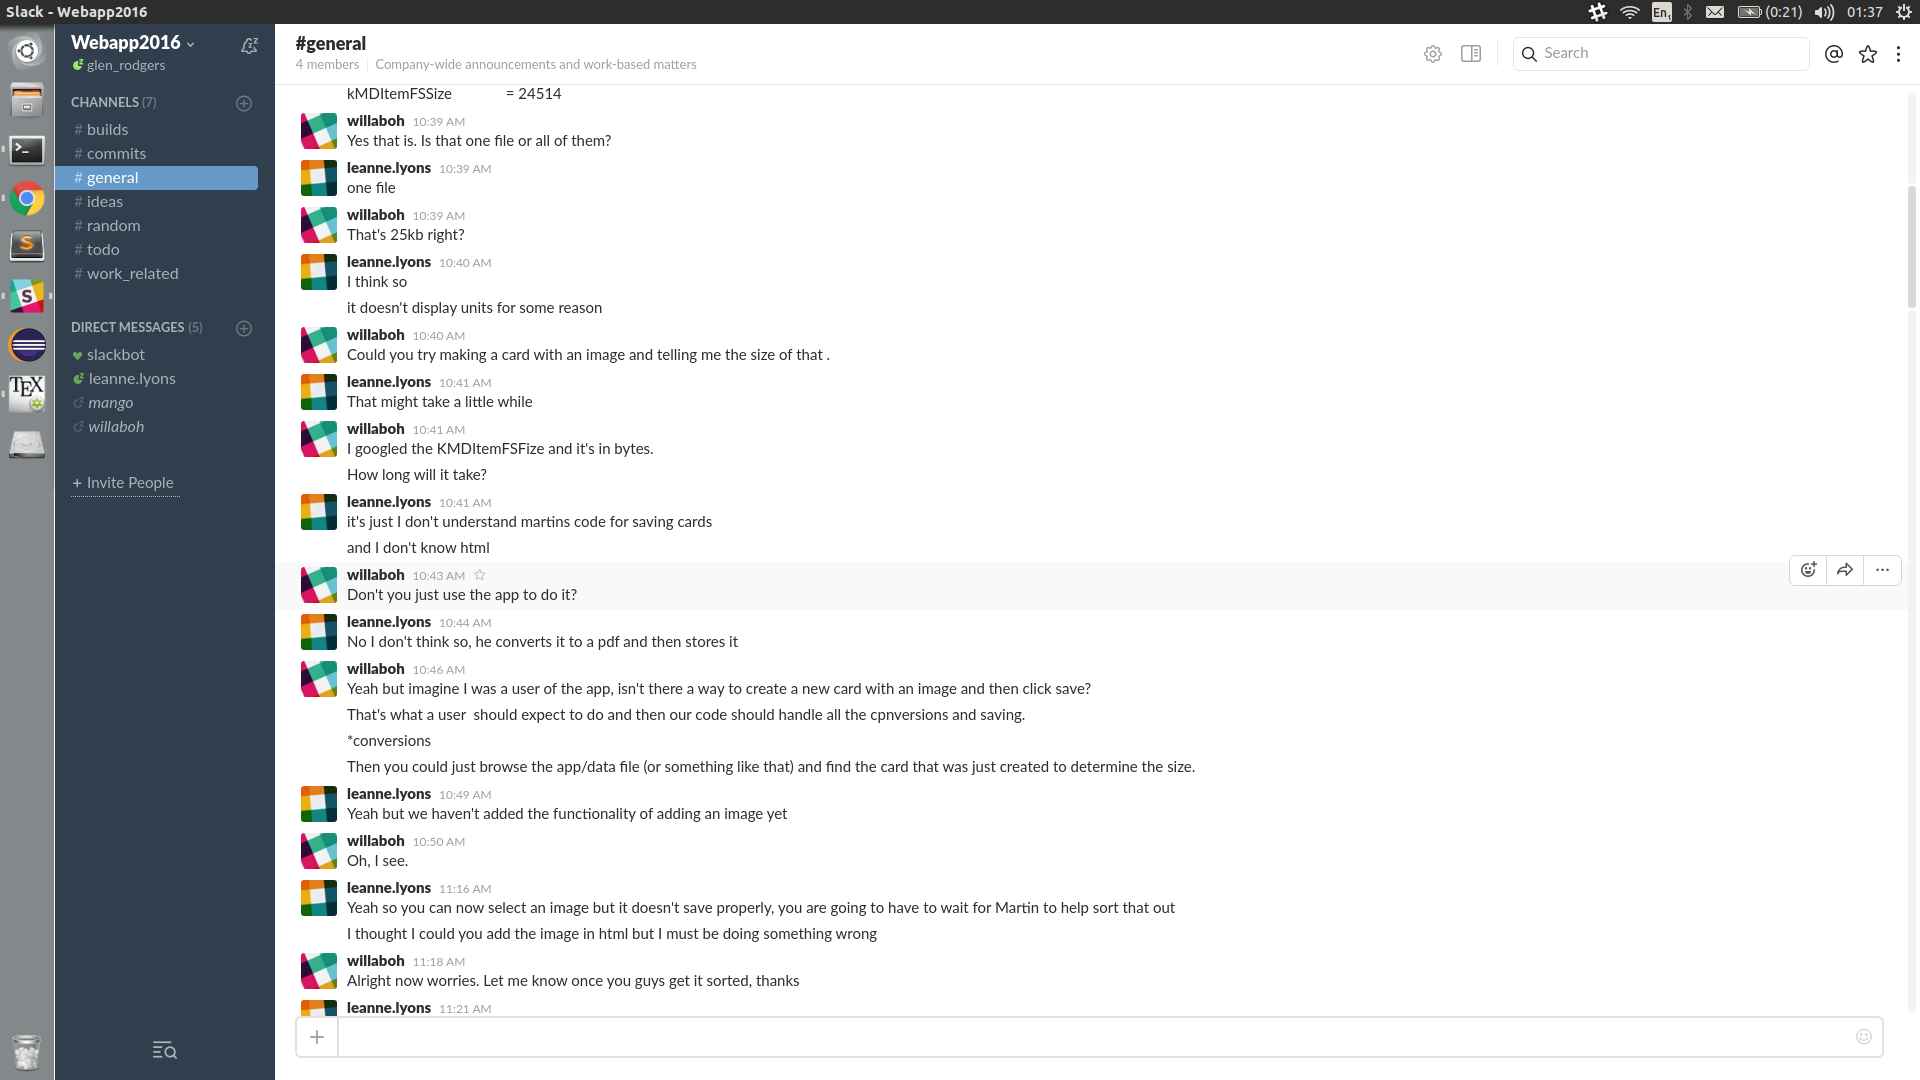
\includegraphics[scale=0.1]{slackend.png} 
  \label{fig:sub1}
\end{subfigure}%
\begin{subfigure}{.5\textwidth}
  \centering
  	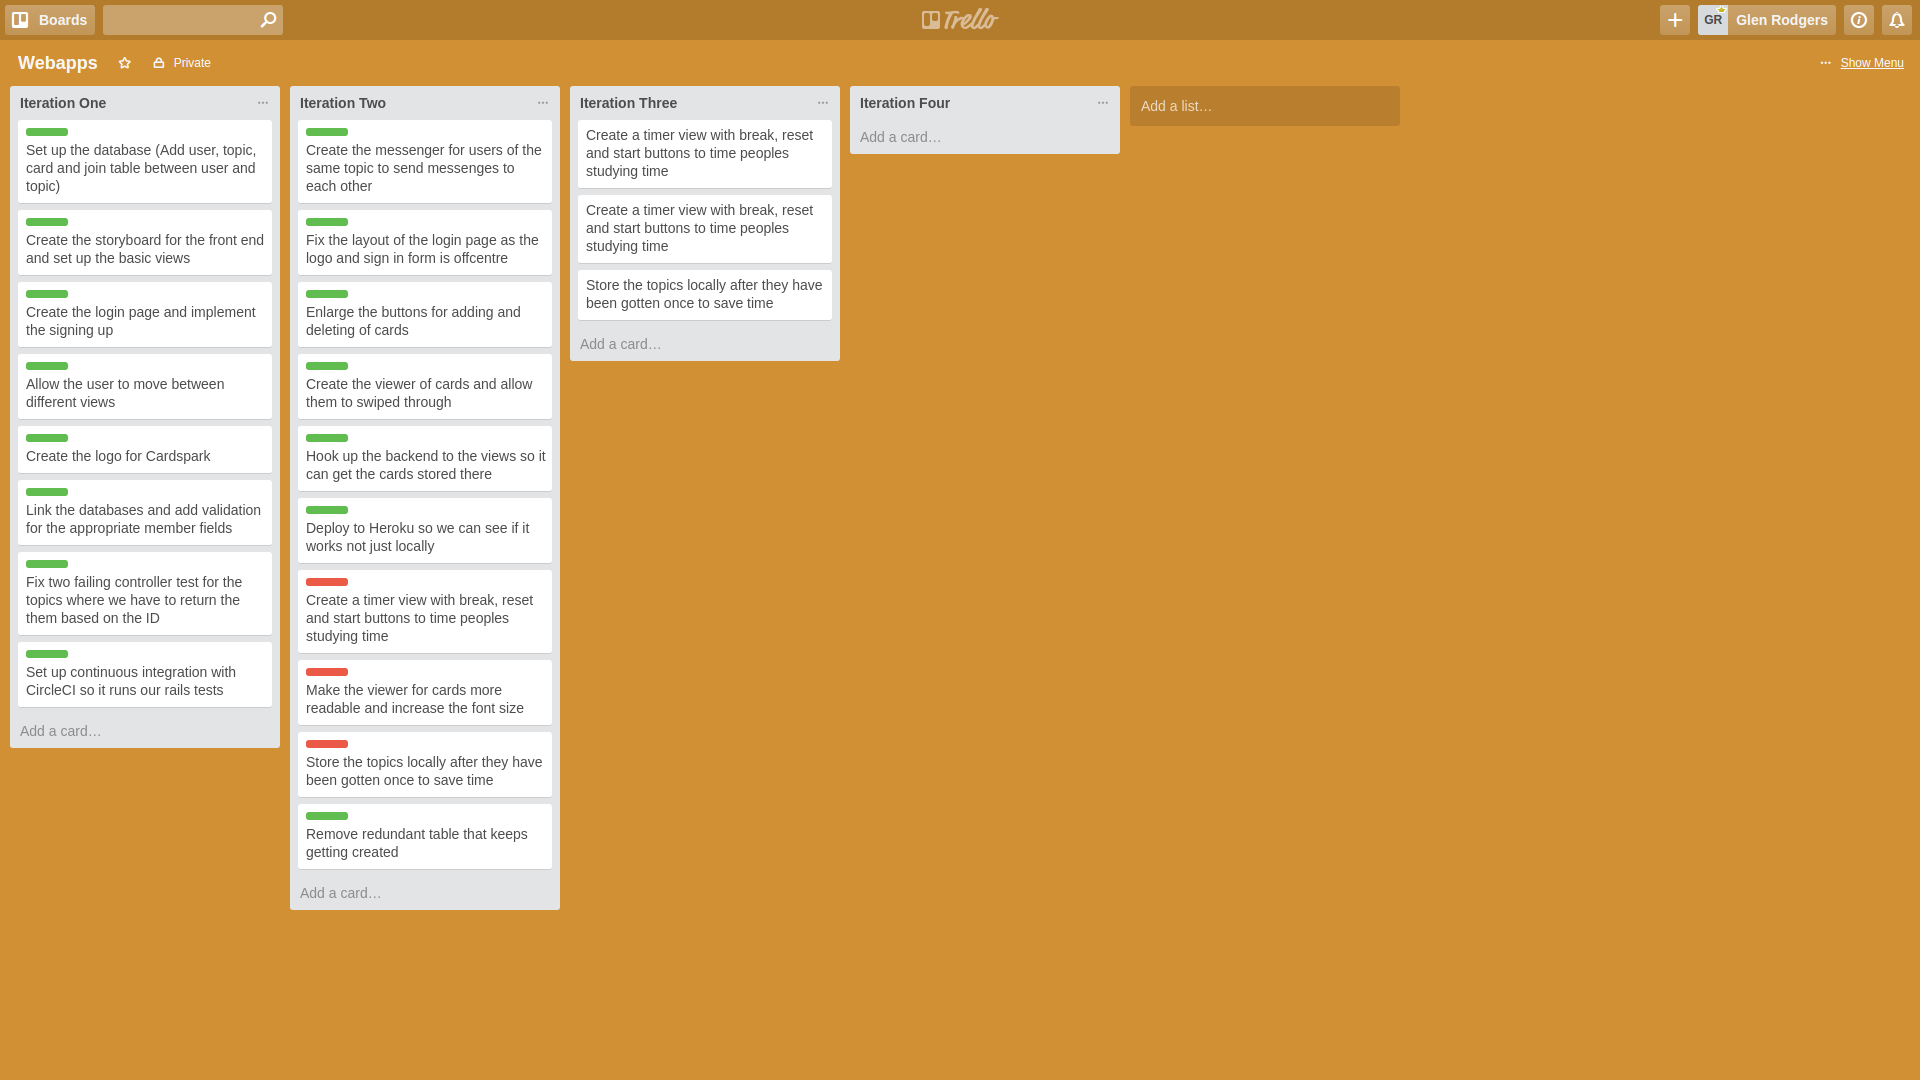
\includegraphics[scale=0.1]{iterationlast.png}  
  \label{fig:sub2}
\end{subfigure}
\label{fig:test}
\end{figure}



\end{document}